\documentclass{beamer}
\mode<presentation>
{
  \usepackage{theme/theme}
  \setbeamercovered{transparent}
}

\usepackage{amsmath,amssymb,amsfonts}
\usepackage{times}
\usepackage{graphicx}
\usepackage{fancyvrb}
\usepackage{array}
\usepackage{colortbl}
\usepackage{tabularx}
\usepackage{fontspec}
\usepackage{minted}
\usepackage{libs/tikz-uml}

% Uncomment me when you need to insert code
\usepackage{color}
\usepackage{listings}
% End Code

% End Header

% Titlepage
\newcommand{\maintitle}{L1. Lab Introduction}
\title{\maintitle}
\author{Enterprise Software Architectures}
\institute
{
  Bachelor's Degree in Computer Engineering
}
\date{Academic year 2025/26}
% End Titlepage

\AtBeginSection[]{
  \begin{frame}
    \centering
    \begin{beamercolorbox}[sep=8pt,center]{title}
      \usebeamerfont{title}\insertsectionhead
    \end{beamercolorbox}
  \end{frame}
}

% Slides
\begin{document}

\begin{frame}
  \titlepage
\end{frame}

\begin{frame}
  \frametitle{\maintitle}
  \tableofcontents[subsectionstyle=show]
\end{frame}

\section{Block A - Introduction to Enterprise Software}
\begin{frame}
  \frametitle{Quick history lesson}

  \begin{columns}[T,onlytextwidth]
    \column{0.5\textwidth}
    \centering
    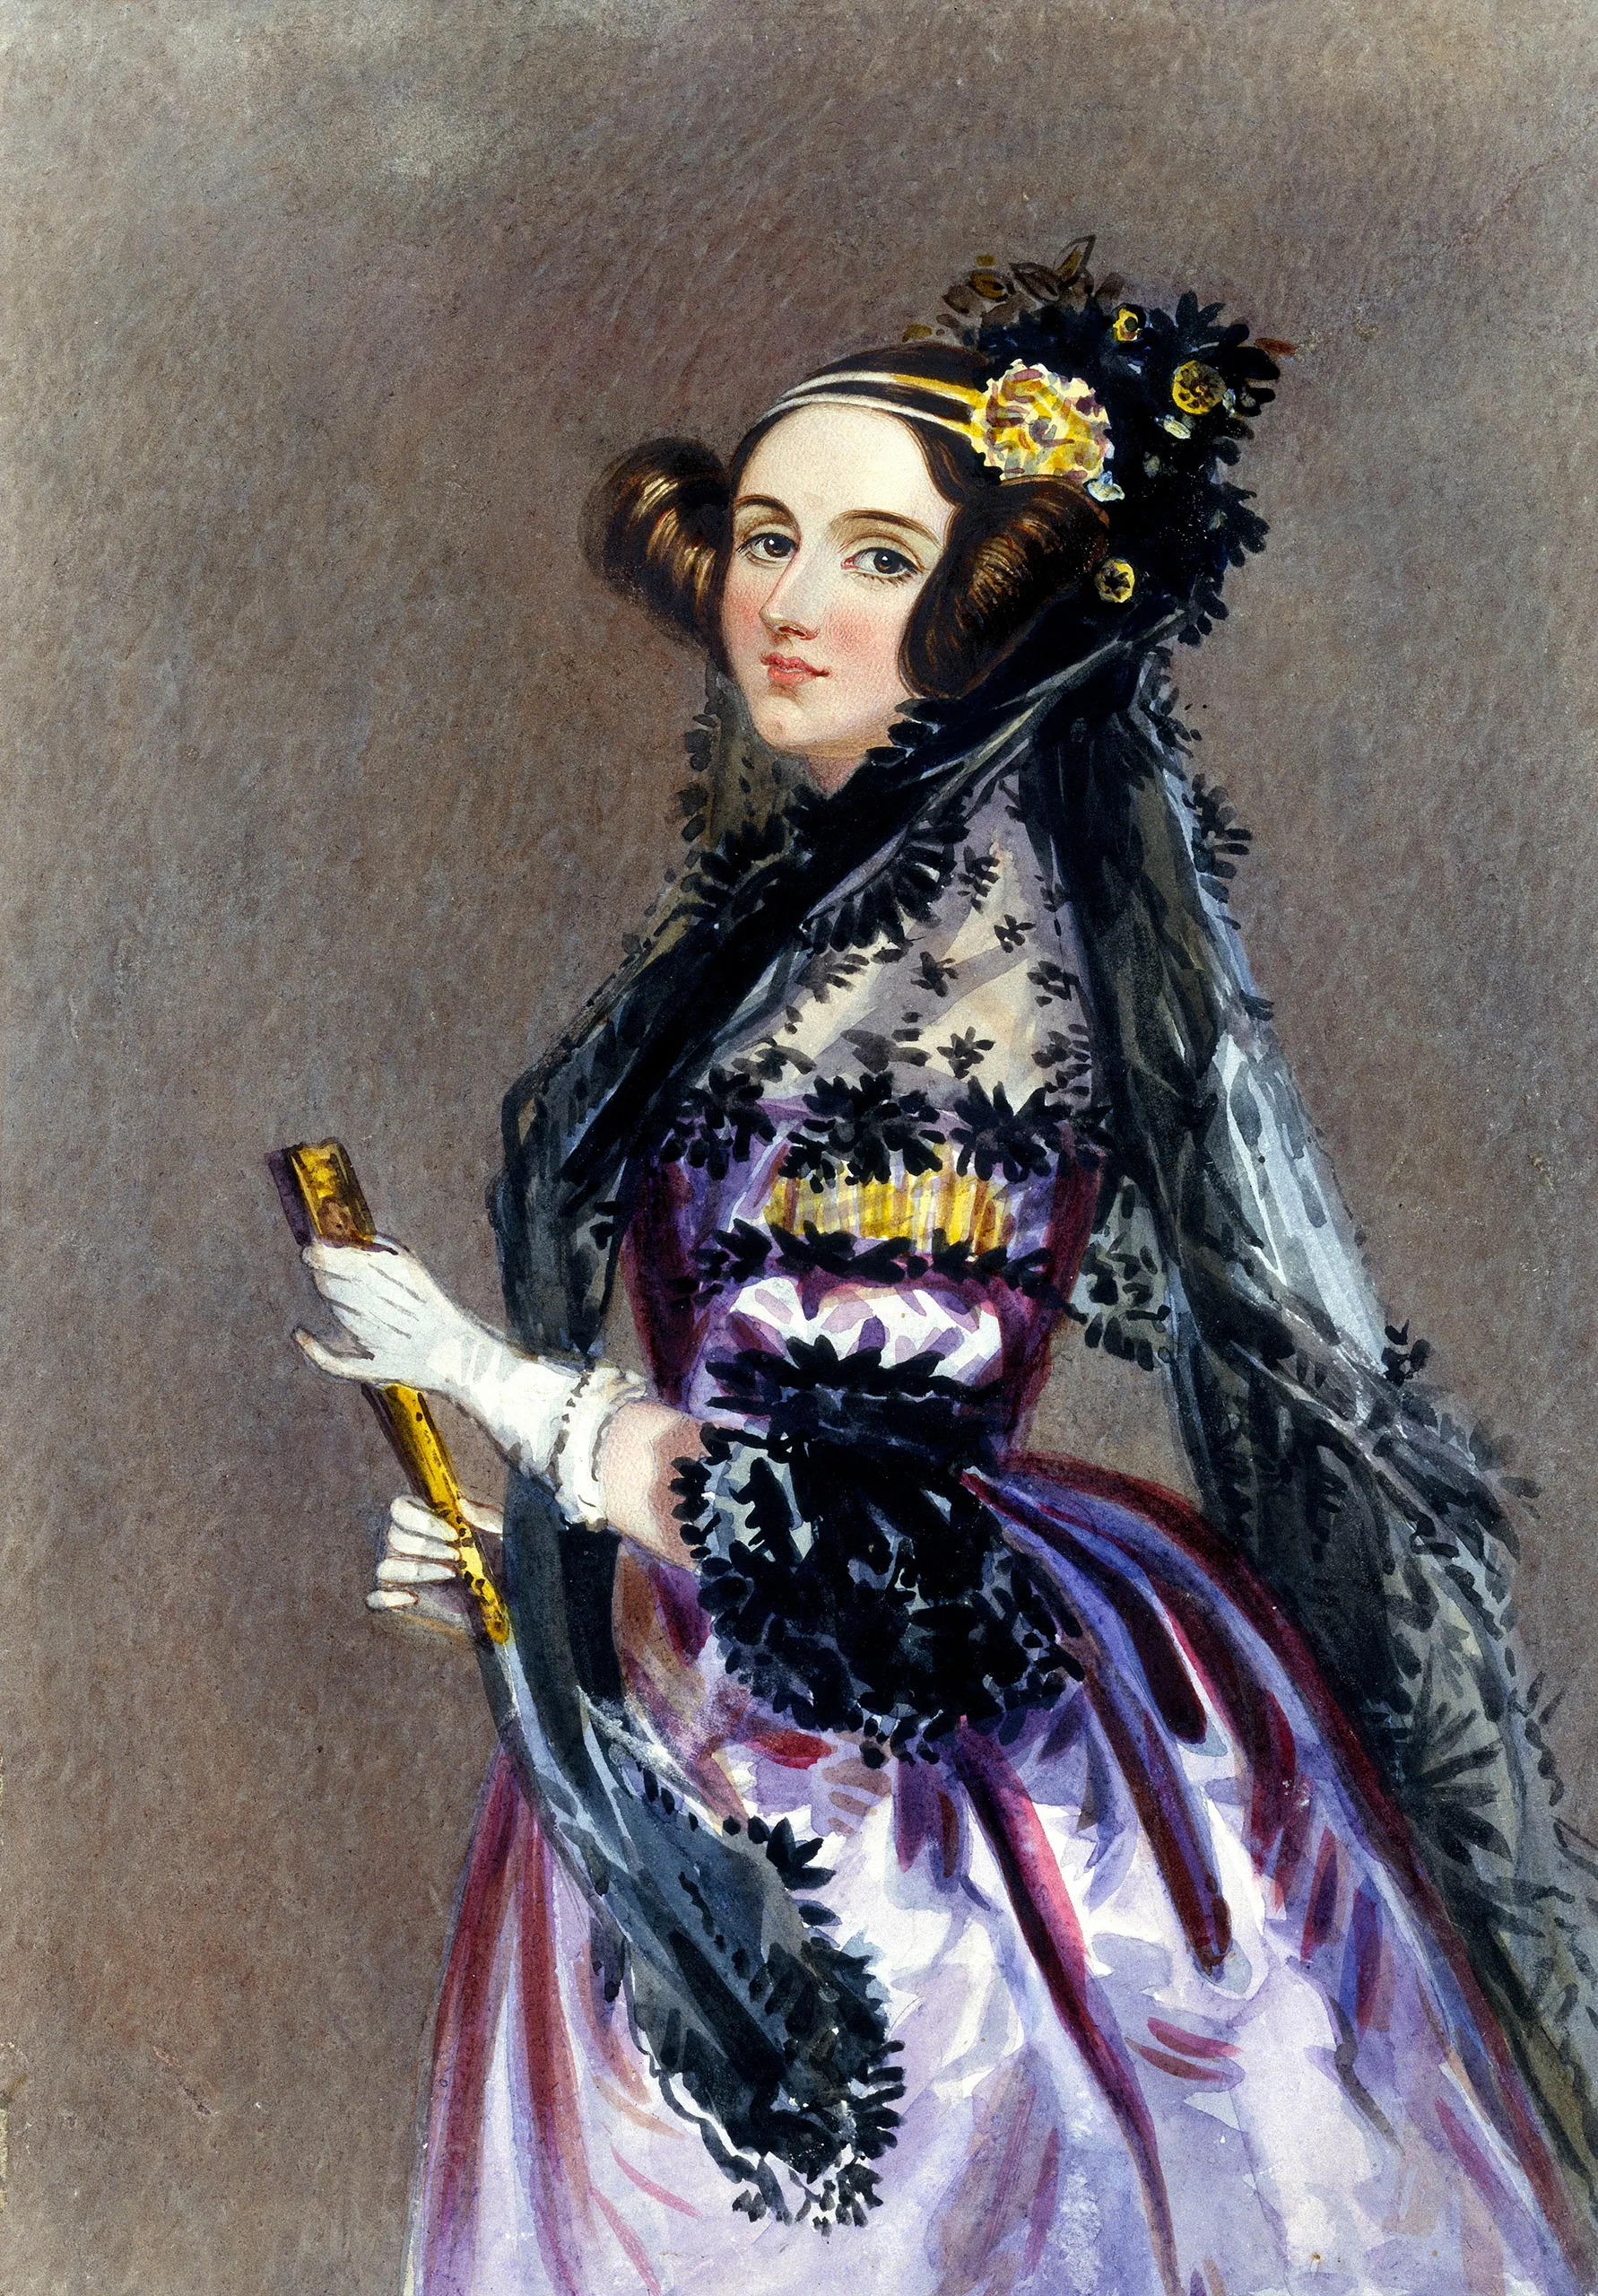
\includegraphics[height=0.7\textheight]{images/L1/lovelace.png}

    \visible<2->{\vspace{0.5ex}\scriptsize Ada Lovelace (first programmer)}
    \column{0.5\textwidth}
    \centering
    \includegraphics[height=0.7\textheight]{images/L1/hamilton.jpg}

    \visible<2->{\vspace{0.5ex}\scriptsize Margaret Hamilton (first software engineer)}
  \end{columns}
\end{frame}

\begin{frame}
  \frametitle{What is Enterprise Software?}

  \begin{itemize}
    \item \textbf{Lovelace} wrote the first algorithms for Babbage's Analytical Engine. They were \textbf{simple programs} and were meant as an intellectual exercise or proof of concept.

      \vfill

    \item \textbf{Hamilton} and her \textbf{MIT team} developed the on-board flight software for NASA's Apollo Guidance Computer. It was the \textbf{most complex} and \textbf{safest} software ever written at the time.\footnote{Fun fact: the full source code is publicly available on GitHub: \url{https://github.com/chrislgarry/Apollo-11}}
  \end{itemize}

\end{frame}

\begin{frame}
  \frametitle{What is Enterprise Software?}

  You are not Ada Lovelace, you are Margaret Hamilton.
  \newline

  \begin{itemize}
    \item Software Engineers work in \textbf{teams} to solve \textbf{complex problems} with \textbf{real stakes} (potentially human lives).
    \item Complex software problems require different \textbf{architecture patterns} and \textbf{development strategies} compared to simple software.
  \end{itemize}

\end{frame}

\begin{frame}
  \frametitle{Software Engineers are Engineers}

  \begin{columns}
    \column{0.7\textwidth}
    Engineers...
    \begin{itemize}
      \item Don't reinvent the wheel: use \textbf{standards} (IEEE, ISO...), \textbf{patterns} and \textbf{good practices}.
      \item Care about long-term \textbf{reliability} and \textbf{performance}.
      \item Work within \textbf{requirements} and \textbf{budgets}.
      \item Use \textbf{formal diagrams} to communicate.
      \item Build prototypes and run controlled experiments.
    \end{itemize}

    \column{0.3\textwidth}
    \centering
    \begin{tikzpicture}
      \umlclass{SoftwareEngineer}{}{}
      \umlclass[x=0,y=2]{Engineer}{}{}

      \umlinherit[geometry=-|]{SoftwareEngineer}{Engineer}
    \end{tikzpicture}

  \end{columns}

\end{frame}

\begin{frame}
  \frametitle{The difference between a \textit{Programmer} and a \textit{Software Engineer}}

  \begin{columns}
    \column{0.5\textwidth}
    \centering
    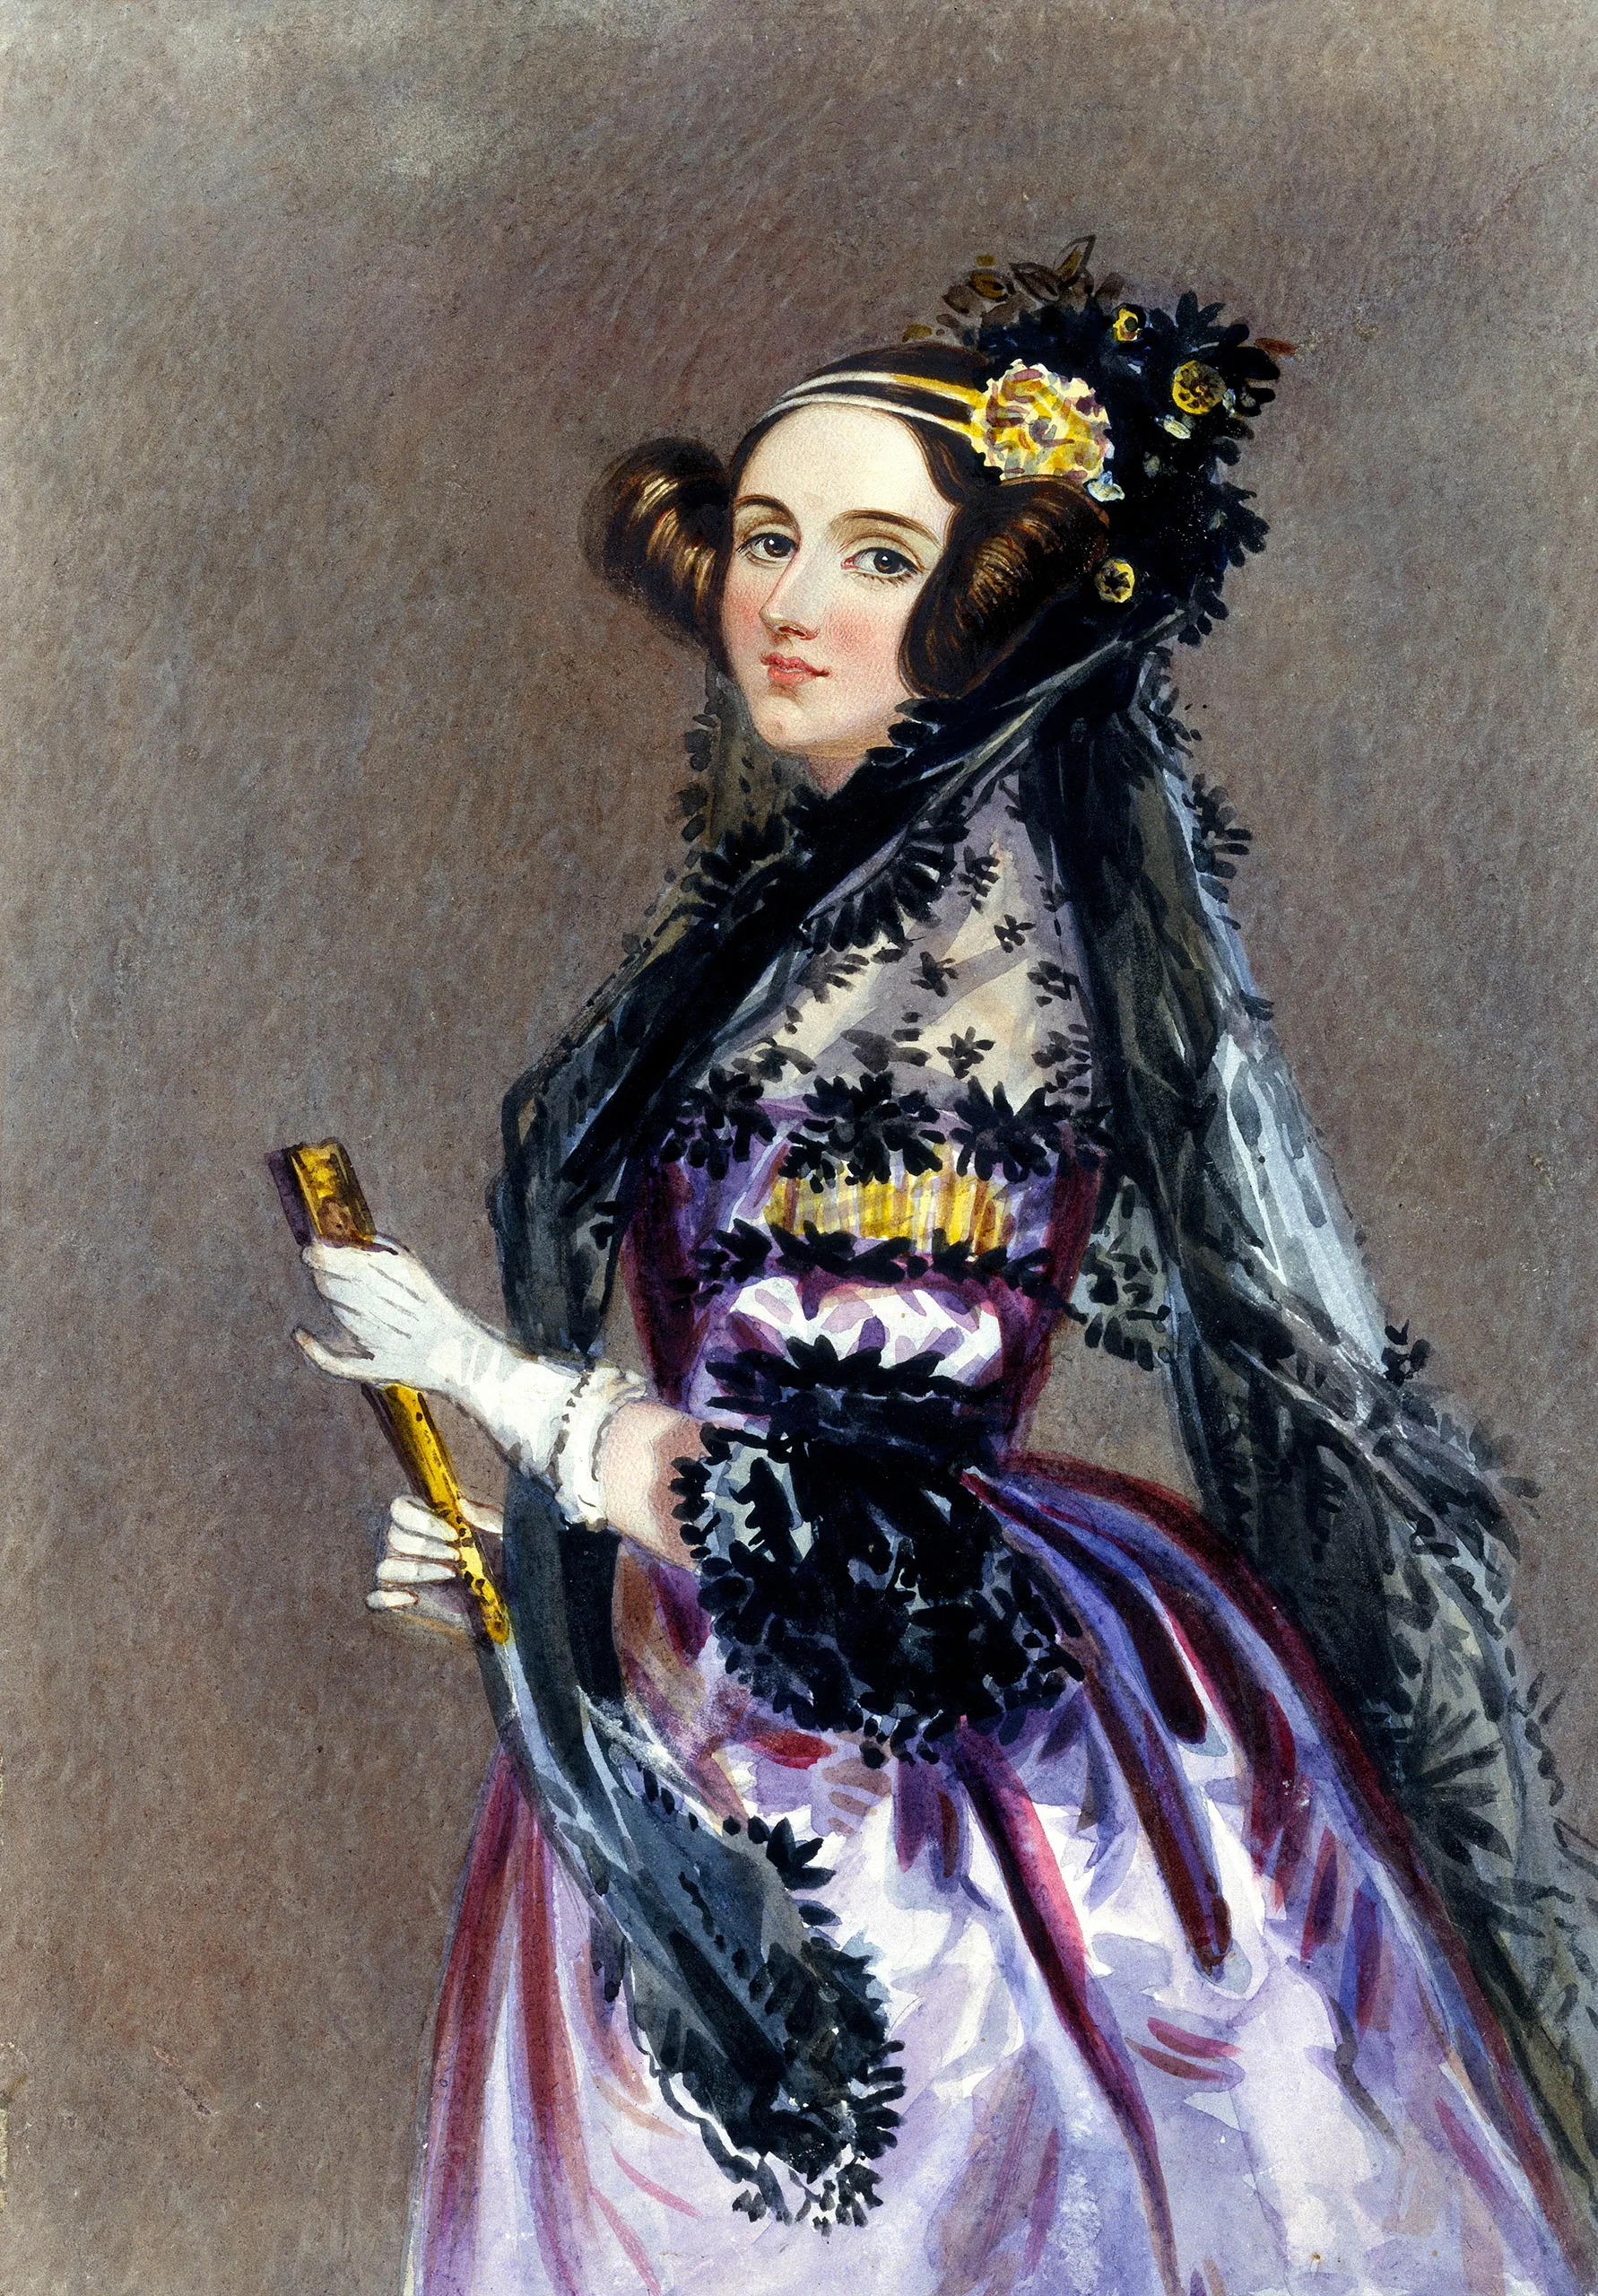
\includegraphics[height=0.7\textheight]{images/L1/lovelace.png}

    \column{0.5\textwidth}
    \centering
    {\textit{\huge "Wow! Your code is so clever and creative!"}}
    
    {\color{white} . \newline}
    
    \visible<2->{\raggedright\textbf{\huge Thanks!}}
  \end{columns}
\end{frame}

\begin{frame}
  \frametitle{The difference between a \textit{Programmer} and a \textit{Software Engineer}}

  \begin{columns}
    \column{0.5\textwidth}
    \centering
    {\textit{\huge "Wow! Your code is so clever and creative!"}}
    
    {\color{white} . \newline}

    \visible<2->{\raggedleft\textbf{\huge Then I must have made a terrible job!}}

    \column{0.5\textwidth}
    \centering
    \includegraphics[height=0.7\textheight]{images/L1/hamilton.jpg}

  \end{columns}
\end{frame}

\begin{frame}

  {\textit{\Large "Debugging is twice as hard as writing the code in the first place. Therefore, if you write the code as cleverly as possible, you are, by definition, not smart enough to debug it."}}

  \raggedleft - Brian Kernighan

\end{frame}

\section{Block B - Project overview}
\subsection{Basic requirements}
\begin{frame}
  \frametitle{Basic requirements}
  \begin{itemize}
    \item Our client wants the frontend to be a web-app.
      \begin{itemize}
        \item This is good for us. We can write one web-app instead of creating native applications for Windows, Android, iOS, etc.
      \end{itemize}
    \item We need to persist information about the users, teams, etc.
      \begin{itemize}
        \item We'll need a database.
      \end{itemize}
    \item The entire system must be performant, reliable, and secure.
  \end{itemize}
\end{frame}

\subsection{Physical architecture}
\begin{frame}
  \frametitle{Physical architecture}
  We'll use a simple and battle-tested Client-Server architecture:
  \begin{figure}
    \includegraphics[scale=1]{images/L1/PhysicalArch1.pdf}
    \caption{Physical architecture high-level overview}
  \end{figure}
\end{frame}

\begin{frame}
  \frametitle{Choosing technologies}

  We'll pick the most widely used technologies for each area:
  \url{https://survey.stackoverflow.co/2025/technology/}
  \newline
  \newline
  Other decisions to make:
  \begin{itemize}
    \item Client-Side Rendering vs Server-Side Rendering
    \item REST vs GraphQL
      \begin{itemize}
        \item \url{https://blog.postman.com/graphql-vs-rest/}
      \end{itemize}
  \end{itemize}
\end{frame}

\begin{frame}
  \frametitle{Physical architecture \& Used technologies}
  \begin{figure}
    \includegraphics[scale=1]{images/L1/PhysicalArch2.pdf}
    \caption{Physical architecture high-level overview}
  \end{figure}
\end{frame}

\begin{frame}
  \frametitle{Source code hosting}
  Code will be hosted on \href{https://github.com/UdL-EPS-SoftArch-Igualada}{\textbf{GitHub}}.
  \newline

  We will use some static analysis tools to keep code quality high and speed up code review:
  \begin{itemize}
    \item \textbf{udl-softarch[bot]}: custom GitHub automation bot (more on that next week).
    \item \textbf{\href{https://www.sonarsource.com/products/sonarqube/}{SonarQube}}: The de-facto standard for static code analysis.
    \item \textbf{\href{https://www.coderabbit.ai/}{CodeRabbit}}: AI-powered code review assistant (let's see how it performs).
  \end{itemize}
\end{frame}

\section{Block C - Project structure \& demo}

\begin{frame}
  \frametitle{Project structure}

  Configuration files (which you can probably ignore):
  \begin{itemize}
    \item \texttt{pom.xml}: Maven project configuration and dependencies.
    \item \texttt{MainApplication.java}: Main application entry point.
    \item \texttt{config/*}: Spring components and configuration.
  \end{itemize}

\end{frame}

\begin{frame}
  \frametitle{Project structure}

  \textbf{Important files for development:}
  \begin{itemize}
    \item \texttt{controller/*}: Web layer. This is where REST endpoints can be manually created.
    \item \texttt{domain/*}: \textbf{Domain layer.} This contains a Java implementation of the domain entities (and their corresponding business logic).
    \item \texttt{repository/*}: Persistence layer. Contains Spring Data interfaces for storing/loading entities from/to the database.
    \item \texttt{handler/*}: Hooks that perform additional work on certain lifecycle events from the persistence layer.
  \end{itemize}

\end{frame}

\begin{frame}
  \frametitle{Project structure}

  \textbf{Important files for testing:}
  \begin{itemize}
    \item \texttt{test/resources/features/*}: Cucumber features (BDD).
    \item \texttt{test/java/.../steps/*}: Java implementation of steps that can be used in the feature files.
  \end{itemize}
  You don't need to worry about them until next week.

\end{frame}

\section{A word from our sponsor}
\begin{frame}
  \frametitle{... a sponsor?!}
  

  \begin{columns}
    \column{0.6\textwidth}
    Our application will be deployed in a \textbf{real production environment}.

    My employer has agreed to generously cover the full cost of our backend server and domain name.
    \newline

    \begin{block}{About our server}
      The server is located in Nuremberg, Germany. It has 2 CPU cores, 4 GB of RAM and 40 GB of SSD storage.
    \end{block}

    \column{0.4\textwidth}
    \begin{figure}
      \includegraphics[width=1\textwidth]{images/L1/server.jpg}
      \caption{A server room. Source: \href{https://commons.wikimedia.org/wiki/File:CERN_Server.jpg}{Wikimedia Commons}}
    \end{figure}

  \end{columns}

\end{frame}

\begin{frame}
  \frametitle{What is LogiCommerce?}

  \begin{figure}
    \includegraphics[height=0.6\textheight]{images/L1/logicommerce.png}
  \end{figure}
  \begin{columns}
    \column{0.15\textwidth}
        \href{https://www.munichsports.com/}{\includegraphics[width=1\textwidth]{images/L1/munich.png}}
    \column{0.15\textwidth}
        \href{https://www.vicens.com/}{\includegraphics[width=1\textwidth]{images/L1/torrons-vicens.png}}
    \column{0.15\textwidth}
        \href{https://www.milan.es/es}{\includegraphics[width=1\textwidth]{images/L1/milan.pdf}}
  \end{columns}

\end{frame}

\begin{frame}
  \frametitle{Our tech stack}

  \begin{columns}
    \column{0.5\textwidth}
      \begin{itemize}
        \item Java (Jakarta EE)
        \item MySQL, MongoDB, Redis
        \item Amazon Web Services
        \item PHP
        \item Lucee / ColdFusion
        \item Python
        \item React + TypeScript
      \end{itemize}

    \column{0.5\textwidth}
      \begin{figure}
        \includegraphics[width=1\textwidth]{images/L1/code.jpg}
        \caption{Source: \href{https://www.pexels.com/photo/close-up-photo-of-programming-of-codes-546819}{Luis Gomes at Pexels (license: Public Domain)}}
      \end{figure}
    
  \end{columns}

\end{frame}

\section{Work assignment}
\begin{frame}
  \frametitle{Work assignment}

  \begin{enumerate}
    \item Make sure you have completed the "Group creation" test. Wait to get access to the "UdL-EPS-SoftArch-Igualada" GitHub organization.
    \item \textbf{Fork} the backend (Java) repository. Be careful \textbf{not} to fork the \textit{template} repository.
    \item Have a look around the repository.
  \end{enumerate}
\end{frame}

\end{document}
